\ProvidesFile{IMprocedure.tex}[v1.0.0]
\primaryStart[InstallationProcedure]{The~Installation~Procedure}
\secondaryStart{Macintosh~OS~X}
The files needed for an \mplusm{} installation are all contained within the
\asCode{M+M.pkg} file; note that Administrator privileges are needed to perform the
installation.
\tertiaryStart{Installing~The~Packages}
After obtaining the \asCode{M+M.pkg} file, open it by double--clicking, at which point the
\asEmphCode{Introduction} page is presented.
\objScaledPicture{Installer01.eps}{0.75}

Click on the \asBoldCode{Continue} button to proceed.
\newpage
The \asEmphCode{Read~Me} page will now appear, which describes what software tools are
needed if you wish to do development with \mplusm{} -- these are not part of the
\asCode{M+M.pkg} file and will need to be installed separately.
\objScaledPicture{Installer02.eps}{0.75}
Determine whether you have the software tools mentioned and click on the
\asBoldCode{Continue} button to proceed, or the \asBoldCode{Print\textellipsis} or
\asBoldCode{Save\textellipsis} to record the other software tools that you would need for
development.
\newpage
The \asEmphCode{License} page will now appear; please read it and click on the
\asBoldCode{Continue} button to proceed, or the \asBoldCode{Print\textellipsis} or
\asBoldCode{Save\textellipsis} buttons to record the license.
\objScaledPicture{Installer03.eps}{0.75}
Once you click on the \asBoldCode{Continue} button, you will be asked to confirm that you
agree to the license; click on the \asBoldCode{Agree} button to accept the license, on the
\asBoldCode{Disagree} button to stop the installation process or on the
\asBoldCode{Read~License} button to go back to the \asEmphCode{License} page.
If you agree to the license, the installation will proceed.
\objScaledPicture{Installer04.eps}{0.75}
\newpage
The \asEmphCode{Installation~Type} page will now appear -- at this point you can select
which items will be installed and where to install them.
\objScaledPicture{Installer05.eps}{0.75}
Click on the \asBoldCode{Change~Install~Location\textellipsis} button to specify the disk
drive where the \mplusm{} packages will be installed, on the \asBoldCode{Customize} button
if you wish to select the packages that will be installed, on the \asBoldCode{Go~Back}
button if you would like to review the license and on the \asBoldCode{Install} button if
you are ready to proceed with the installation.
\newpage
If you clicked on the \asBoldCode{Change~Install~Location\textellipsis} button on the
\asEmphCode{Installation~Type} page, the\\
\asEmphCode{Select~a~Destination} page will appear.
You can select any disk drive that contains the Macintosh OS X operating system on it.
Typically, only one disk drive is selectable; the current operating system disk will be
selected if there is sufficient space to do the installation.
The amount of disk space required to install the packages that you have selected will also
appear.
\objScaledPicture{Installer05a.eps}{0.75}
Select a disk drive by clicking on it and then click on the \asBoldCode{Continue} button
to return to the \asEmphCode{Installation~Type} page.
\newpage
If you clicked on the \asBoldCode{Customize} button on the \asEmphCode{Installation~Type}
page, the \asEmphCode{Custom~Install} page will appear.
\objScaledPicture{Installer06.eps}{0.75}
Click on the \asBoldCode{Standard~Install} button to return to the
\asEmphCode{Installation~Type} page, with just the \asCode{Core} package selected, on the
\asBoldCode{Go~Back} button to return to the \asEmphCode{Installation~Type} page with the
current selections and on the \asBoldCode{Install} button to proceed with the installation.
\newpage
If you clicked on the \asCode{Core} package, a description of the package appears.
The \asCode{Core} package is always installed -- if you have an existing \mplusm{}
installation, the Action shown will be `Upgrade', not `Install'.
\objScaledPicture{Installer06a.eps}{0.75}
\newpage
If you clicked on the \asCode{Developer} package, a description of the package appears.
The \asCode{Developer} package is optional -- if you have an existing \mplusm{}
installation that includes the \asCode{Developer} package, the Action shown will be
`Upgrade', not `Install'.
The default Action is to `Skip' the installation of the \asCode{Developer} package.
\objScaledPicture{Installer06b.eps}{0.75}
Note that the amount of disk space required to the install the packages will be adjusted
to reflect if the \asCode{Developer} package has been selected for installation.
\newpage
Clicking on the \asBoldCode{Install} button on the \asEmphCode{Installation~Type} page
will result in a page being displayed which requests an administrator name and password.
\objScaledPicture{Installer07.eps}{0.75}
Clicking on the \asBoldCode{Cancel} button will return you to the
\asEmphCode{Installation~Type} page; entering a valid administrator name and password and
clicking on the \asBoldCode{Install~Software} button will result in a series of pages
being displayed, reflecting the installation progress.
\newpage
Once the installation completes, the \asEmphCode{Summary} page will appear.
\objScaledPicture{Installer08.eps}{0.75}
Click on the \asBoldCode{Close} button to exit from the installer.
\newpage
\tertiaryEnd{}
\tertiaryStart{Testing~The~Installation}
Open the \asCode{Terminal} program and enter the following:
\outputBegin{}
yarp server
\outputEnd{}
If you see the following, there was another copy of \yarp{} already running on the system
and you will need to stop it before continuing:
\outputBegin{}
\begin{verbatim}
__   __ _    ____  ____  
\ \ / // \  |  _ \|  _ \ 
 \ V // _ \ | |_) | |_) |
  | |/ ___ \|  _ <|  __/ 
  |_/_/   \_\_| \_\_|    
\end{verbatim}
Call with --help for information on available options\\
Options can be set on command line or in /Users/M\textunderscore{}M/Library/Application\\
\hspace*{5em}Support/yarp/config/yarpserver.conf\\
Using port database:\ :memory:\\
Using subscription database:\ :memory:\\
IP address:\ default\\
Port number:\ 10000\\
yarp:\ Port /root failed to activate at tcp://10.0.1.2:10000 (address conflict)\\
Name server failed to open
\outputEnd{}
If you see the following, the \asCode{Terminal} program was running during the
installation and did not pick up the correct settings:
\outputBegin{}
-bash:\ yarp:\ No such file or directory
\outputEnd{}
Exit from the \asCode{Terminal} program and open it again, so that its settings will be
updated.\\

If you see the following, \yarp{} started correctly, and the \mplusm{} installation can be
confirmed:
\outputBegin{}
\begin{verbatim}
__   __ _    ____  ____  
\ \ / // \  |  _ \|  _ \ 
 \ V // _ \ | |_) | |_) |
  | |/ ___ \|  _ <|  __/ 
  |_/_/   \_\_| \_\_|    
\end{verbatim}
Call with --help for information on available options
Options can be set on command line or in /Users/M\textunderscore{}M/Library/Application\\
\hspace*{5em}Support/yarp/config/yarpserver.conf\\
Using port database:\ :memory:\\
Using subscription database:\ :memory:\\
IP address:\ default\\
Port number:\ 10000\\
yarp:\ Port /root active at tcp://10.0.1.2:10000\\

Registering name server with itself:\\
\hspace*{0.5em}* register "/root" tcp "10.0.1.2" 10000\\
\hspace*{1.6em}+ set "/root" ips "127.0.0.1" "10.0.1.2"\\
\hspace*{1.6em}+ set "/root" process 61856\\
\hspace*{0.5em}* register fallback mcast "224.2.1.1" 10000\\
\hspace*{1.6em}+ set fallback ips "127.0.0.1" "10.0.1.2"\\
\hspace*{1.6em}+ set fallback process 61856\\
Name server can be browsed at http://10.0.1.2:10000/\\

Ok.  Ready!\\
Name server running happily
\outputEnd{}
Once you've confirmed that \yarp{} is running correctly, it's time to start \mplusm{}.
Start another \asCode{Terminal} session or open another tab in the \asCode{Terminal}
application and enter the following:
\outputBegin{}
mpmRegistryService \&
\outputEnd{}
The output similar to the following should appear:
\outputBegin{}
\openSq{}1\closeSq{} 63918\\
registered admin's iMac.\fatUnderscore{}yarpns.\fatUnderscore{}tcp.local.
\outputEnd{}
where `1' will be incremented each time that a process is run in the background, `63918'
will be replaced by the process identifier for the copy of \asCode{mpmRegistryService}
that is running and `admin's iMac' will be replaced by the name of the computer on which
\mplusm{} has been installed.\\

If something similar to the following appears:
\outputBegin{}
\openSq{}1\closeSq{} 64234\\
\openSq{}1\closeSq{}+\hspace*{1em}Done\hspace*{8em}mpmRegistryService
\outputEnd{}
then the \asCode{mpmRegistryService} application was already running when \mplusm{} was
installed, indicating that this was not a new installation but, rather, an upgrade.\\

It will be necessary to stop the earlier copy of \asCode{mpmRegistryService}.
To to this, find the running copy via the command:
\outputBegin{}
ps -ax | grep -i mpm | grep -v grep
\outputEnd{}
A single line of output should appear, similar to:
\outputBegin{}
63918 ttys015   16:42.19 mpmRegistryService
\outputEnd{}
where `63918' will be the process identifier of the already--running copy of
\asCode{mpmRegistryService}.
Enter the following command, replacing `63918' with the first number that appeared in the
output that was just displayed.
\outputBegin{}
kill -s HUP 63918
\outputEnd{}
It should now be possible to issue the `\asCode{mpmRegistryService \&}' command as
described earlier.
\newpage
The last step in testing the \mplusm{} installation is to launch the
\asCode{Channel~Manager} application, which was placed in the \asCode{/Applications}
directory.
You should see something similar to the following:
\objScaledPicture{RunningChannelManager.eps}{0.75}
You now have a test \mplusm{} installation and begin using it for your projects!
\tertiaryEnd{}
\secondaryEnd{}
\newpage
\secondaryStart{Microsoft~Windows}

To install the M+M, simply execute the installer package titled "M+M-1.x.x-win32.exe". Depending on your security settings, you may receive a User Access Warning. Simply click next if that is the case. You will be greeted with the following window:

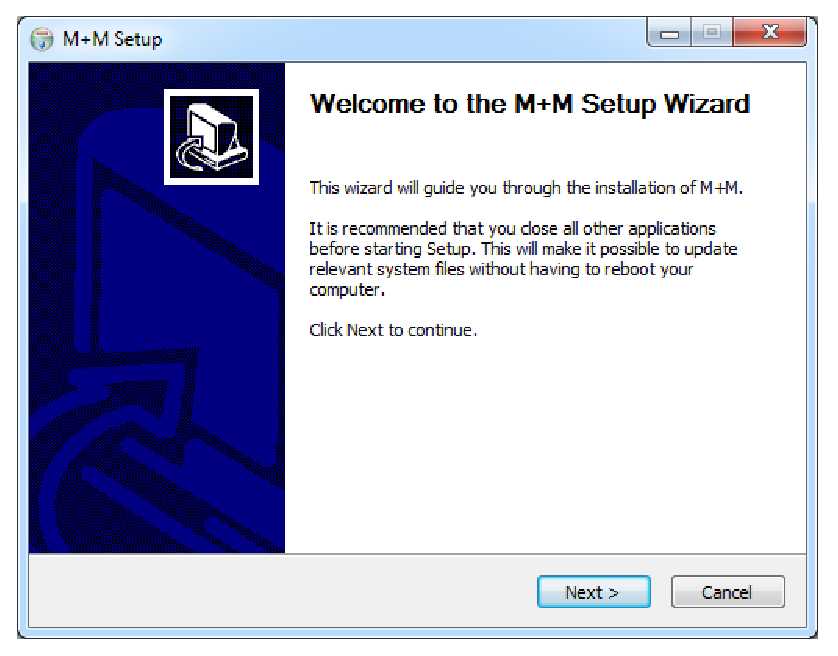
\includegraphics[keepaspectratio=true,scale=0.74]{img/win_install01}

Click "I agree" to proceed.

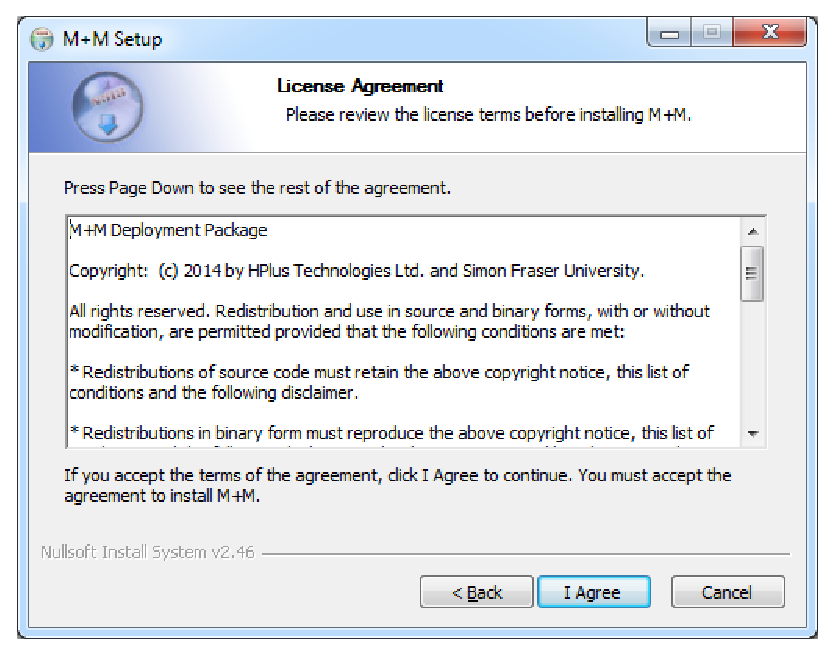
\includegraphics[keepaspectratio=true,scale=0.74]{img/win_install02}

Then, select the destination for the installed files:

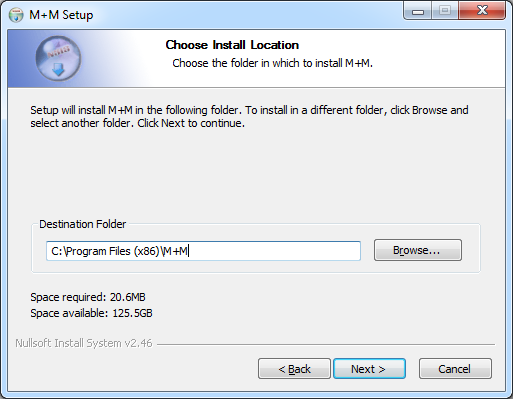
\includegraphics[keepaspectratio=true,scale=0.74]{img/win_install03}


An option to create a Start Menu folder will be provided. Currently this will contain a shortcut to the uninstaller application.

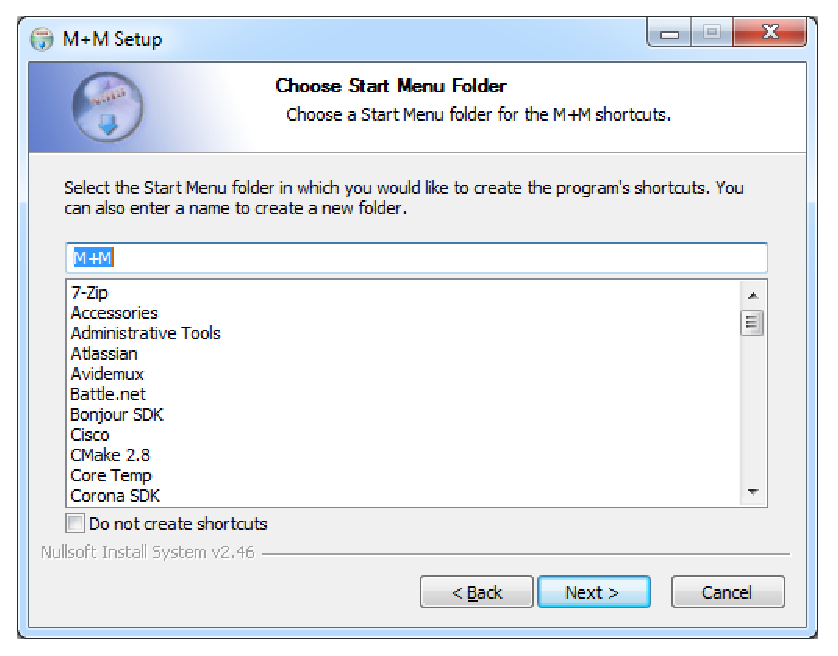
\includegraphics[keepaspectratio=true,scale=0.74]{img/win_install04}

Here you can select the components to be installed. The Minimal Install contains just the libraries, without the example applications.

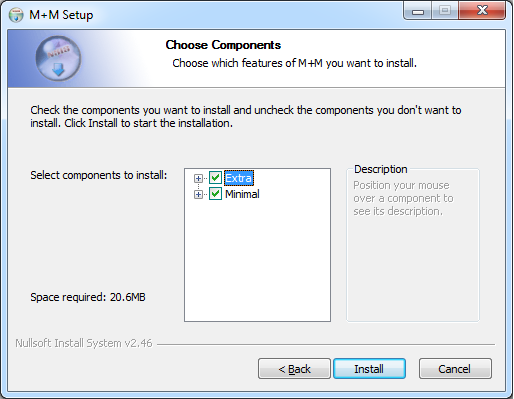
\includegraphics[keepaspectratio=true,scale=0.74]{img/win_install05}

The M+M Library makes use of the Apple Bonjour SDK, and the installer will be launched at this point:

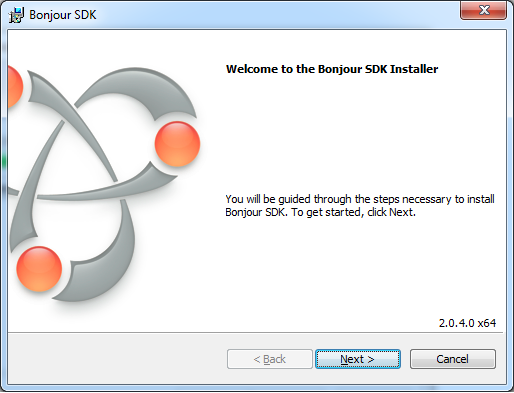
\includegraphics[keepaspectratio=true,scale=0.74]{img/win_install06}

Proceed with the installation of the Bonjour SDK:

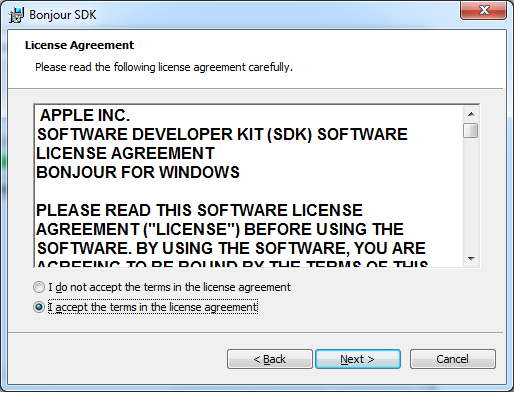
\includegraphics[keepaspectratio=true,scale=0.74]{img/win_install07}

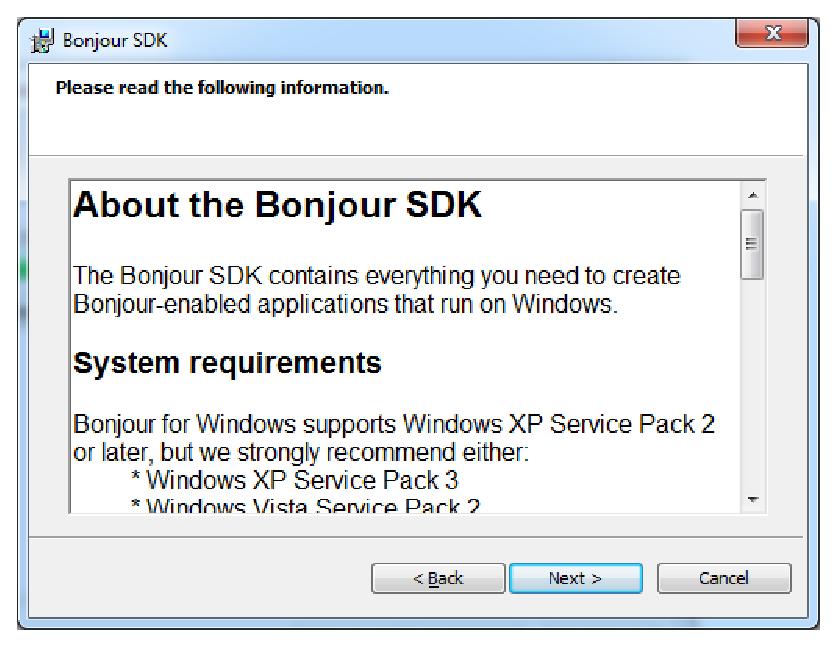
\includegraphics[keepaspectratio=true,scale=0.74]{img/win_install08}

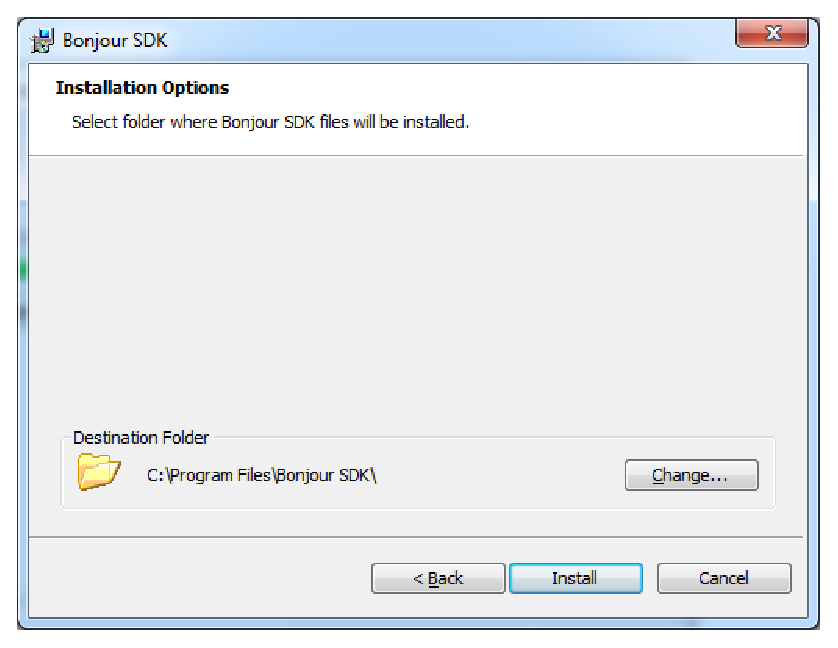
\includegraphics[keepaspectratio=true,scale=0.74]{img/win_install09}

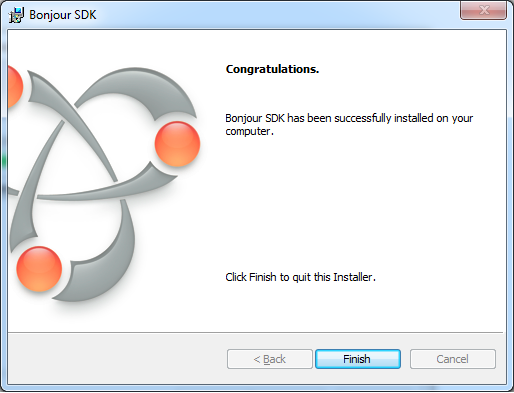
\includegraphics[keepaspectratio=true,scale=0.74]{img/win_install10}

\newpage
This finalizes the installation process:

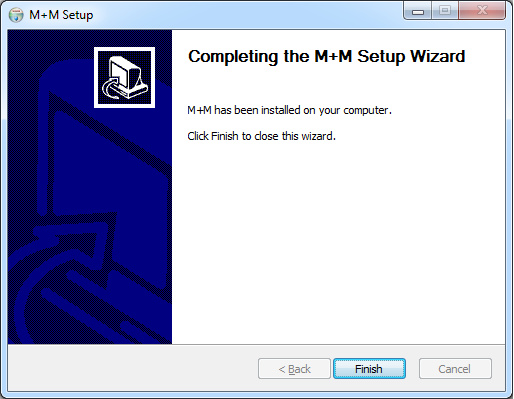
\includegraphics[keepaspectratio=true,scale=0.74]{img/win_install11}

\secondaryEnd{}
\primaryEnd{}
